\documentclass[12pt letter]{report}
\input{../template/preamble}
\input{../template/macros}
\input{../template/letterfonts}

\usepackage{tikz}
\usepackage{hyperref}
\hypersetup{
    colorlinks=true,
    linkcolor=blue,
    filecolor=magenta,      
    urlcolor=cyan,
    pdftitle={Overleaf Example},
    pdfpagemode=FullScreen,
    }

\urlstyle{same}
\usetikzlibrary{automata, positioning, arrows}
\tikzset{
->, % makes the edges directed
% >=stealth’, % makes the arrow heads bold
node distance=3cm, % specifies the minimum distance between two nodes. Change if necessary.
every state/.style={thick, fill=gray!10}, % sets the properties for each ’state’ node
initial text=$ $, % sets the text that appears on the start arrow
}
\usepackage{booktabs}
\usepackage{karnaugh-map}
\usepackage{parskip}
\title{\Huge{Homework 1}}
\author{\huge{Madiba Hudson-Quansah}}
\date{}


\begin{document}
\maketitle
\newpage

\section*{Digital Logic and Design}
\qs{}{
  Design a 4-bit binary multiplier using combinational logic (AND gates and adders). Show the step-by-step process of multiplying two 4-bit binary numbers, 1011 (11 in decimal) and 1101 (13 in decimal).
  Calculation Steps:
  \begin{itemize}
    \item  Perform binary multiplication and explain each step in detail.
    \item  Provide the final product in binary and decimal.
  \end{itemize}
}

\sol{
\[
  \begin{array}{c c c c c c c c c}
           &   &   &   &   & 1 & 0 & 1 & 1 \\
    \times &   &   &   &   & 1 & 1 & 0 & 1 \\
    \hline
           &   &   &   &   & 1 & 0 & 1 & 1 \\ % 1011 times 1, shifted 0 positions
    +      &   &   &   & 0 & 0 & 0 & 0 & 0 \\ % 1011 times 0, shifted 1 position
    +      &   &   & 1 & 0 & 1 & 1 & 0 & 0 \\ % 1011 times 1, shifted 2 positions
    +      &   & 1 & 0 & 1 & 1 & 0 & 0 & 0 \\ % 1011 times 1, shifted 3 positions
    \hline
           & 1 & 0 & 0 & 0 & 1 & 1 & 1 & 1 \\
  \end{array}
\]

Each row in the resulting addition is obtained by multiplying the  multiplicand by each bit of the multiplier, starting
from the least significant bit, i.e. $b_0$ if the multiplier bits are $b_3 b_2 b_1 b_0$, and shifting the result to the
left by the position of the multiplier bit.\\

\noindent Therefore the first row is the result of multiplying 1011 by 1, shifted 0 positions to the left. \\
The second row is the result of multiplying 1011 by 0, shifted 1 position to the left. \\
The third row is the result of multiplying 1011 by 1, shifted 2 positions to the left. \\
And the fourth row is the result of multiplying 1011 by 1, shifted 3 positions to the left. \\

So the final result is:

\[
10001111_{2} = 143_{10}
    \]
  }

\qs{}{
  Use a Karnaugh Map to simplify the following Boolean expression:
  \[
    F \left( A, B, C, D \right) = \displaystyle\sum \left( 0, 2, 6, 8, 10, 12, 14 \right)
  \]
  Draw the K-map and show the process of grouping the minterms. Write the simplified Boolean expression.
}

\sol{
  \begin{figure}[H]
  \centering
  \begin{karnaugh-map}[4][4][1][$CD$][$AB$]
  \minterms{0,2,6,8,10,12,14}
  \autoterms[0]
  \implicantcorner{}
  \implicant{2}{10}
  % \implicant{12}{8}
  \implicantedge{12}{8}{14}{10}
  \end{karnaugh-map}
  \end{figure}
  \[
    F \left( A, B, C, D \right)  = \overline{B}\overline{D} + C \overline{D} + A \overline{D}
  \]
}

\qs{}{
  Design a 3-bit binary up-counter using D flip-flops.
  \begin{itemize}
    \item  Draw the circuit diagram and explain how the counter works.
    \item  Show the state transition table for the counter.
  \end{itemize}
}

\sol{

  \noindent The counter uses three synchronous D flip-flops to store each bit of the current state. The next state of each flip-flop
  past the first one is determined by the  value of the current input ANDED with the past result of the previous
  flip-flop and the result of that XORED with the current state of the flip-flop. The first flip-flop's next state is
  only determined by the XOR of the current input and the current state of flip-flop. This continued accumulation of the
  previous flip-flop's state and the current input is what allows the counter to increment by one for each clock cycle.

  \begin{align*}
    D_1 \left( t + 1 \right) & = \text{Din} \oplus D_1                                                          \\
    D_2 \left( t + 1 \right) & = \left( \text{Din} \cdot D_1   \right) \oplus D_2                               \\
    D_3 \left( t + 1 \right) & =   \left( \left( \text{Din} \cdot D_1 \right) \cdot D_2    \right)   \oplus D_3 \\
    \text{Dout}              & = D_3 D_2 D_1                                                                    \\
  \end{align*}

  \begin{table}[h!]
    \begin{center}
      \begin{tabular}{*{8}{wc{7mm}}} \toprule
        \multicolumn{3}{c}{Current State} &
        \multicolumn{1}{c}{Input}         &
        \multicolumn{3}{c}{Next State}    &
        \multicolumn{1}{c}{Output}                                                                     \\
        \cmidrule(lr){1-4}\cmidrule(lr){5-8}
        $D_3$                             & $D_2$ & $D_1$ & $\text{Din}$ & $D_3$ & $D_2$ & $D_1$ &
        $\text{Dout}$                                                                                  \\ \midrule
        0                                 & 0     & 0     & 0            & 0     & 0     & 0     & 000 \\
        0                                 & 0     & 0     & 1            & 0     & 0     & 1     & 001 \\
        \hline
        0                                 & 0     & 1     & 0            & 0     & 0     & 1     & 001 \\
        0                                 & 0     & 1     & 1            & 0     & 1     & 0     & 010 \\
        \hline
        0                                 & 1     & 0     & 0            & 0     & 1     & 0     & 010 \\
        0                                 & 1     & 0     & 1            & 0     & 1     & 1     & 011 \\
        \hline
        0                                 & 1     & 1     & 0            & 0     & 1     & 1     & 011 \\
        0                                 & 1     & 1     & 1            & 1     & 0     & 0     & 100 \\
        \hline
        1                                 & 0     & 0     & 0            & 1     & 0     & 0     & 100 \\
        1                                 & 0     & 0     & 1            & 1     & 0     & 1     & 101 \\
        \hline
        1                                 & 0     & 1     & 0            & 1     & 0     & 1     & 101 \\
        1                                 & 0     & 1     & 1            & 1     & 1     & 0     & 110 \\
        \hline
        1                                 & 1     & 0     & 0            & 1     & 1     & 0     & 110 \\
        1                                 & 1     & 0     & 1            & 1     & 1     & 1     & 111 \\
        \hline
        1                                 & 1     & 1     & 0            & 1     & 1     & 1     & 111 \\
        1                                 & 1     & 1     & 1            & 0     & 0     & 0     & 000 \\
        \bottomrule
      \end{tabular}
    \end{center}
  \end{table}

}

\qs{}{
  Design a finite state machine (FSM) to detect the sequence "1011" in a stream of binary inputs.
  \begin{itemize}
    \item  Provide the state diagram, state table, and transition logic for the FSM.
    \item  Explain how the FSM detects the sequence.
  \end{itemize}
}

\sol{
  \begin{figure}[H]
    \centering
    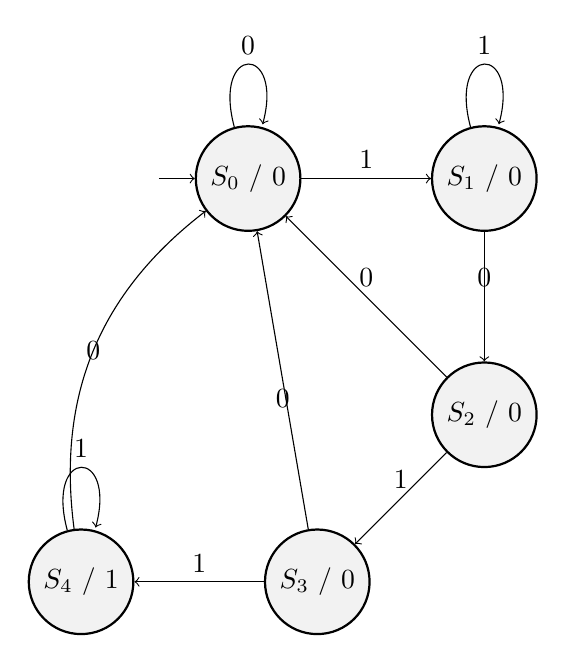
\begin{tikzpicture}
      \node[state, initial] (s0) {$S_0$ / 0};
      \node[state,right of=s0] (s1) {$S_1$ / 0};
      \node[state, below of=s1] (s2) {$S_2$ / 0};
      \node[state, below left of=s2] (s3) {$S_3$ / 0};
      \node[state,  left of=s3] (s4) {$S_4$ / 1};

      \draw
      (s0) edge[loop above] node{0} (s0)
      (s0) edge[above] node{1} (s1)

      (s1) edge[loop above] node{1} (s1)
      (s1) edge[above] node{0} (s2)

      (s2) edge[above] node{0} (s0)
      (s2) edge[above] node{1} (s3)

      (s3) edge[below] node{0} (s0)
      (s3) edge[above] node{1} (s4)

      (s4) edge[loop above] node{1} (s4)
      (s4) edge[bend left] node{0} (s0)
      ;
    \end{tikzpicture}
  \end{figure}

  \begin{table}[h!]
    \begin{center}
      \begin{tabular}{*{4}{wc{15mm}}} \toprule
        \multicolumn{2}{c}{Inputs}     &
        \multicolumn{1}{c}{Next State} &
        \multicolumn{1}{c}{Output}                         \\
        \cmidrule(lr){1-2}
        Present State                  & Input &       &   \\ \midrule
        $S_0$                          & 0     & $S_0$ & 0 \\
        $S_0$                          & 1     & $S_1$ & 0 \\

        $S_1$                          & 0     & $S_2$ & 0 \\
        $S_1$                          & 1     & $S_1$ & 0 \\

        $S_2$                          & 0     & $S_0$ & 0 \\
        $S_2$                          & 1     & $S_3$ & 0 \\

        $S_3$                          & 0     & $S_0$ & 0 \\
        $S_3$                          & 1     & $S_4$ & 0 \\

        $S_4$                          & 0     & $S_0$ & 1 \\
        $S_4$                          & 1     & $S_4$ & 1 \\
        \bottomrule
      \end{tabular}
    \end{center}
  \end{table}


  The FSM detects the sequence by representing each bit the desired sequence as state and changing states depending
  on the input bits read from the bit stream. When the FSM reaches the final state, it outputs a 1 to indicate that the
  sequence has been detected. If the next input bit matches the expected bit for the sequence the FSM transitions to the
  next state, however, if an incorrect bit is found, the FSM transitions back to an earlier state, potentially the
  initial state or a partial match state. This ensures that the FSM continuously scans for the sequence even after
  partial matches.
}

\section*{Computer Systems Architecture}

\qs{}{
  A non-pipelined processor completes an instruction in 15 ns. A pipelined version of the processor breaks the instruction execution into 5 stages, with each stage taking 4 ns. Assuming no pipeline stalls:
  \begin{itemize}
    \item  Calculate the speedup gained by using pipelining.
    \item  Discuss the performance implications if stalls occur in the pipeline.
  \end{itemize}
}

\sol{
  \begin{enumerate}
    \item For the non-pipelined processor the time to complete a single instruction is 15ns. Breaking a single
          instruction execution into 5 stages, each of 4ns results in one execution taking $5 \times 4 = 20ns$. \\
          However, the subsequent instructions will be completed asynchronously / in overlapping stages after the first instruction.
          This means the effective time for each instruction is 4ns after the initial instruction. Therefore, the time
          needed for $n$ instructions in the non-pipelined processor is:
          \[
            \text{Time}_S = 15 \times n
          \]
          And the pipelined:
          \[
            \text{Time}_A = 20 + \left( n - 1 \right)  \times 4
          \]
          The speedup for a single instruction $n = 1$:
          \[
            S = \frac{\text{Time}_ S}{\text{Time}_A} = \frac{15}{20} = 0.75
          \]
          This is actually a slowdown of $0.75$ for a single instruction but for $n > 1$, the speedup is:
          \begin{align*}
            S                      & = \frac{15n}{4n + 16} \\
            \lim_{n \to \infty}  S & = \frac{15}{4}        \\
                                   & = 3.75                \\
          \end{align*}
          So, a speedup of $3.75$ or $375\%$ is achieved for a large number of instructions.
    \item If a stall occurs, this slows down the pipeline and reduces the speedup. The time taken for each
          instruction is increased by the number of cycles the pipeline is stalled. This means the speedup is reduced
          by the number of cycles the pipeline is stalled.
  \end{enumerate}
}

\qs{}{
  Discuss three energy-efficient computing techniques that can be applied in modern processors to reduce power consumption while maintaining performance.
  \begin{itemize}
    \item  Explain each technique in detail, providing examples of their real-world applications.
    \item  Discuss the trade-offs between energy savings and performance.
  \end{itemize}
}

\sol{
  \begin{enumerate}
    \item
          \begin{description}
            \item[Dynamic Voltage and Frequency Scaling (DVFS)] - This technique dynamically adjusts the voltage and
                  frequency a processor operates based on the current load the processor is processing. During idle
                  periods / low load DVFS reduces both the max voltage a processor can draw and the max frequency it can attain,
                  leading to significantly less power draw. However, the voltage drawn and max frequency can
                  increase at high workloads as needed. One real-world example is its use in Qualcomm's Snapdragon series of ARM
                  processors. These processors are usually used in mobile devices, which makes the need for increased
                  battery life great, and DVFS can reduce the CPU's power draw, which is often one of the most power-heavy components of a mobile device.
            \item[Power Gating] - This technique involves selectively disabling power to idle sections of a
                  processor shutting down unused sections of the CPU to reduce power consumption. This technique is
                  used in modern multi-core processor architectures such as Intel's Core i7 series of processors and
                  AMD's Threadripper series.
            \item[Clock Gating] - This technique involves selectively stopping the clock signal to the idle section of
                  a processor, reducing the computations the processor does in total.  Since the clock signal consumes
                  considerable power through its continuous toggling, disabling it in idle components can
                  reduce dynamic and switching power. This technique is also used in Intel and AMD chips to save
                  power in caches, buses and FPUs.
          \end{description}
    \item In pursuit of higher processing speeds, the cost is often increased power draw. Faster clock rates mean
          more frequent transistor switching, which increases power draw. Powering down idle components can
          reduce power draw but also slows response times when those components are reactivated, as they require some
          time to power up.

  \end{enumerate}
}

\qs{}{
  Compare the performance of a single-threaded processor versus a multithreaded processor for a workload with 100,000 instructions. Assume the single-threaded processor takes 5 ns per instruction, and the multithreaded processor can switch between two threads every 3 ns.
  \begin{itemize}
    \item  Calculate the time taken by each processor to complete the workload.
    \item  Discuss the impact of multithreading on performance and resource utilization.
  \end{itemize}
}

\sol{
  \begin{enumerate}
    \item The total time taken by the single-threaded processor is:
          \[
            \text{Time}_S = 100 000 \times 5 = 500 000 \text{ ns}
          \]
          The multithreaded processor can switch between two threads every 3ns, this means that the time taken to
          complete one instruction is 3ns. The time taken to complete the workload is:
          \[
            \text{Time}_M = 100 000 \times 3 = 300 000 \text{ ns}
          \]
          Assuming no overheads or stalls.
    \item
          \begin{description}
            \item[Performance]  - The multithreaded processor can complete the same number of instructions as the
                  single-threaded processor in less time, making the multithreaded processors more performant with a speedup
                  of:
                  \[
                    S = \frac{5000000}{3000000} = \frac{5}{3} = 1.67
                  \]
                  $167\%$
            \item[Resource Utilization] - The multithreaded processor can utilize the CPU more efficiently by
                  switching between threads when one thread is stalled or waiting for data. This means the CPU can do more work in the same time, making it more resource-efficient.
          \end{description}
  \end{enumerate}
}

\section*{Energy Efficiency}

\qs{}{
  The dynamic power consumption in a CMOS circuit is given by $P = C V^2 f$, where C is the capacitance, V is the voltage, and f is the frequency. Suppose the capacitance is 5 pF, the voltage is 1.8 V, and the frequency is 2 GHz.
  \begin{itemize}
    \item  Calculate the dynamic power consumption of the circuit.
    \item  Discuss the impact of reducing voltage and frequency on power consumption and performance.
  \end{itemize}
}

\sol{
  \begin{enumerate}
    \item
          \begin{align*}
            P & = 5 \times 1.8^2 \times 2 \\
              & = 32.4 \text{ mW}         \\
          \end{align*}
    \item
          Reducing the voltage going to a circuit and the frequency of the circuit reduces the circuit's power consumption. This is because the
          power consumption of a circuit is proportional to the square of the voltage and frequency of the circuit,
          meaning that with every decrease in any of these units, the power consumption decreases. However, reducing the voltage and frequency of a circuit
          reduces the circuit's performance, as the circuit's performance is proportional to the voltage and frequency of the circuit.
  \end{enumerate}
}

\qs{}{
  Data centres are known for high energy consumption, especially due to cooling requirements. Propose a strategy to reduce the energy consumption of a data center, focusing on both hardware and software solutions.
  \begin{itemize}
    \item  Discuss energy-efficient hardware technologies and cooling systems.
    \item  Suggest software-based strategies like virtualization and dynamic resource allocation to optimize energy usage.
  \end{itemize}
}

\sol{
  \begin{enumerate}
    \item
          \begin{description}
            \item[Low-Power Processors] - Using processors with lower power consumption and energy-saving modes, reduces
                  heat generation reducing cooling requirements and power consumption. Such energy saving modes include DVFS.
            \item[Liquid Cooling] - By circulating a liquid coolant directly through systems, cooling can be done more
                  efficiently as liquids have a higher heat capacity than air, meaning they can absorb more heat before
                  needing to be cooled.
            \item[Solid State Drives (SSDs)] - SSDs consume less power and produce less heat compared to traditional
                  hard drives.
          \end{description}
    \item
          \begin{description}
            \item[Virtualization] - Virtualization allows running multiple (virtual) machines onto fewer physical
                  servers, reducing the number of servers required, reducing hardware power and cooling demands.
            \item[Dynamic Resource Allocation] - Dynamic resource allocation strategies such as dynamic scaling, where
                  computing resources are adjusted in real-time in relation to system load, and load balancing where
                  workloads are efficiently distributed across servers reducing over reliance on specific machines,
                  reduce hardware power consumption needs, thereby reducing cooling needs.
          \end{description}
  \end{enumerate}
}

\qs{}{
  Dynamic Voltage and Frequency Scaling (DVFS) is a technique used to adjust the power consumption of a processor based
  on workload demand. Assume a processor operates at a voltage of 1.2 V and frequency of 3 GHz. If DVFS reduces the
  voltage by 15\% and frequency by 20\%, calculate the new power consumption using the formula
  \[
    P = C V^2 f
  \]
  \begin{itemize}
    \item  Show the step-by-step calculation for the new power consumption.
    \item  Discuss the trade-offs between energy savings and performance loss when applying DVFS.
  \end{itemize}
}

\sol{
  \begin{enumerate}
    \item
          Assuming $C = 1$
          \begin{align*}
            P_1 & = \left( 1.2 \times 0.85 \right) ^2 \times \left( 3 \times 0.8 \right) \\
                & = 2.49696 \text{ mW}                                                   \\
          \end{align*}
    \item  When the voltage draw is reduced the amount of power used by circuit is reduced but the performance of the circuit is also reduced. This is because the performance of a circuit is proportional to the voltage and frequency of the circuit. Therefore, reducing the voltage and frequency of a circuit reduces the circuit's performance.
  \end{enumerate}
}



\end{document}
